\newif\ifvimbug
\vimbugfalse

\ifvimbug
\begin{document}
\fi


\subsection{Kubische B-Splines und de Boor Algorithmus (6 Punkte)}
\subsubsection{3 Punkte}
\begin{tikzpicture}[grow=left,
level 1/.style={sibling distance=15mm},edge from parent/.style={-,draw},>=latex, level 3/.style={edge from child/.style={->,draw},sibling distance=15mm}]

\node[root] {$B_{-2}^3(t)$}
     child {node[level 2] (c1) {$B_{-2}^2(t)$}
       child {node[level 2] (c21) {$B_{-1}^1(t)$}
       		child {node[level 2] (c211) {$B_{0}^0(t)$}}
             }
       }
       child {node[level 2] (c2) {$B_{-1}^2(t)$}
       child {node[level 2] (c21) {}
       		}
       child {node[level 2] (c22) {$B_{0}^1(t)$}
              			child {node[level 2] (c3111) {$B_{1}^0(t)$}}
             }
       };

\end{tikzpicture}\\
\hspace{-1.0cm}
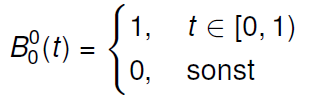
\includegraphics[scale=0.5]{1aB00.PNG}
\\
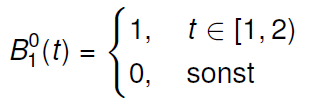
\includegraphics[scale=0.5]{1aB01.PNG}
\\
\hspace{-0.9cm}
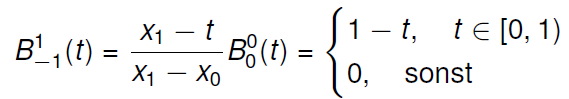
\includegraphics[scale=0.5]{1aB1-1.PNG}
\\
\hspace{-2.7cm}
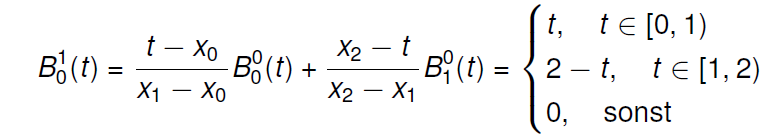
\includegraphics[scale=0.5]{1aB10.PNG}
\\
\hspace{-1.4cm}
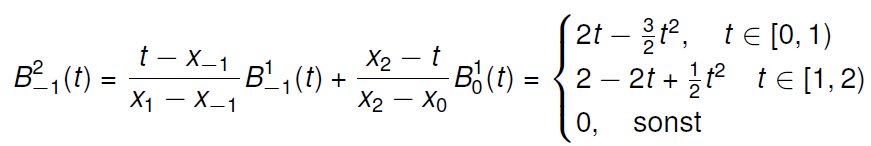
\includegraphics[scale=0.5]{1aB2-1.PNG}
\\
$B_{-2}^2(t) = \frac{x_{-2+2+1}-t}{x_{-2+2+1}-x_{-2+1}} * B_{-1}^1(t) = 1-t * B_{-1}^1(t) = \begin{cases}
    t^2 - 2t + 1       & \quad \text{if } t \in [0,1)\\
    0  & \quad \text{sonst}
  \end{cases}$
\\
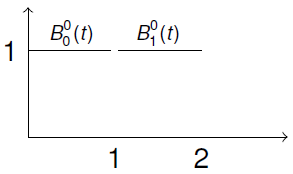
\includegraphics[scale=0.7]{GB0.PNG}
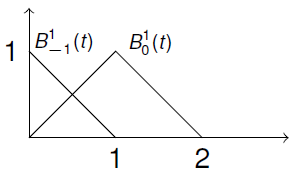
\includegraphics[scale=0.7]{GB1.PNG}
\\
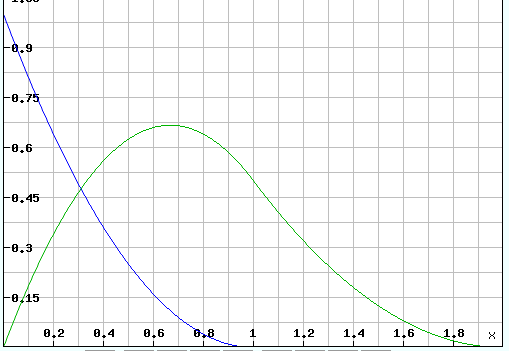
\includegraphics[scale=0.7]{GB2.PNG}
Blau enstpricht $B_{-2}^2(t)$ und grün $B_{-1}^2(t)$



\subsubsection{3 Punkte}

1) $1.5 \in [x_{j}, x_{j+1}) \implies 1.5 \in [1,2) \implies j=1$
\\
2) $i = j - q,...,j \implies i = -2,...,1$
\\
3) $\lambda_{1,i}^{[l]}(\xi) = \frac{x_{i+q+1-l}- \xi}{x_{i+q+1-l}-x_i}$
und $\lambda_{2,i}^{[l]}(\xi) = 1 - \lambda_{1,i}^{[l]}(\xi)$
\\
4)
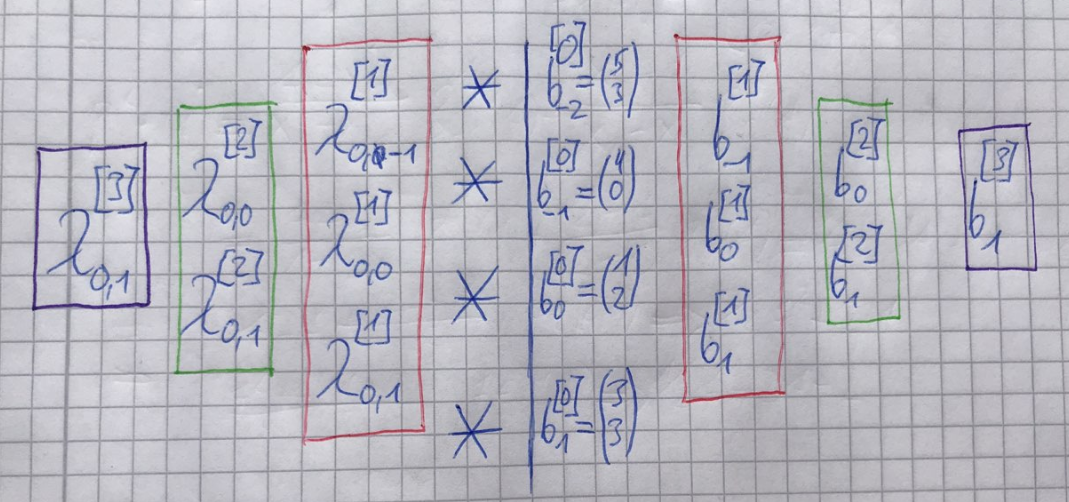
\includegraphics[scale=0.5]{1b)1.PNG}
\\
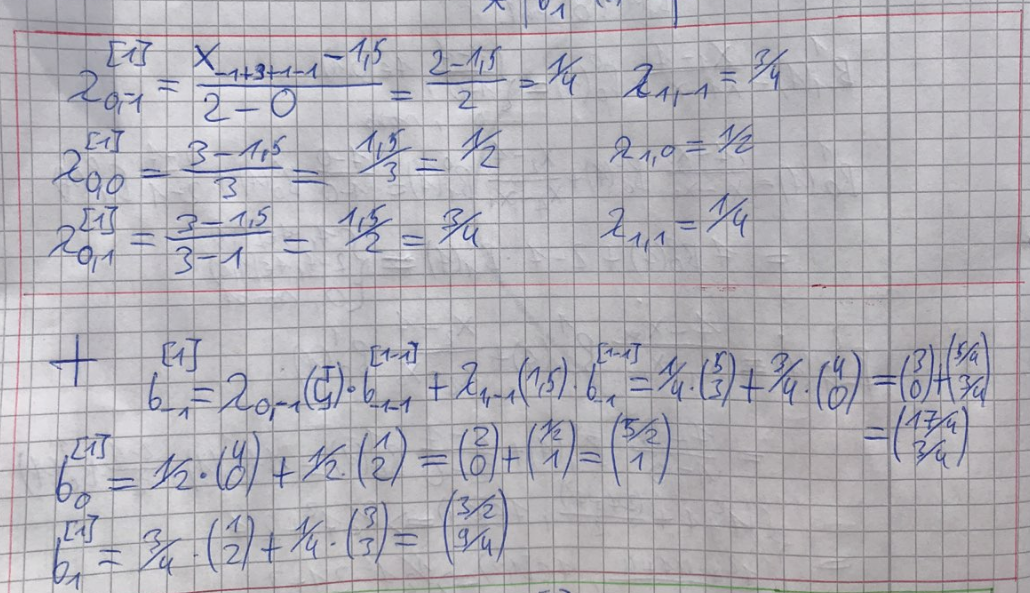
\includegraphics[scale=0.5]{1b)2.PNG}
\\
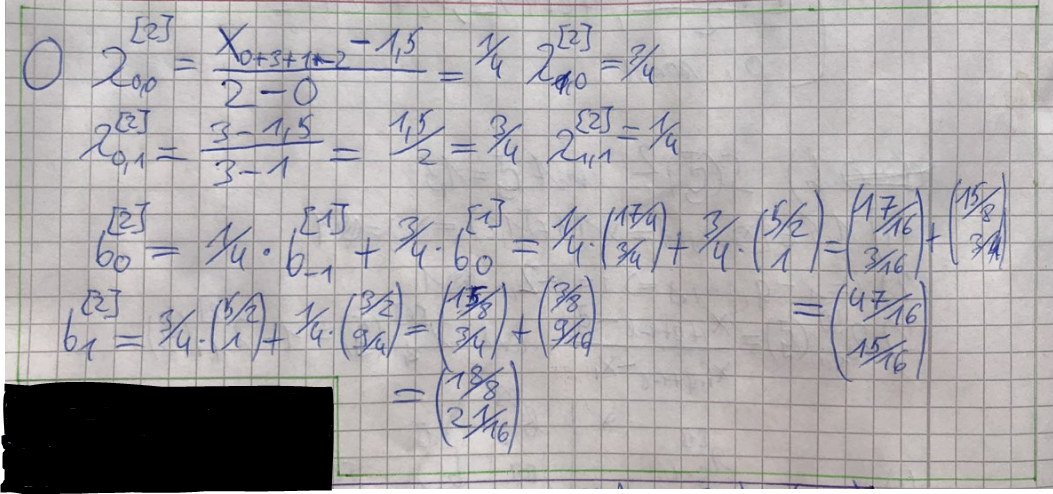
\includegraphics[scale=0.5]{1b)3.PNG}
\\
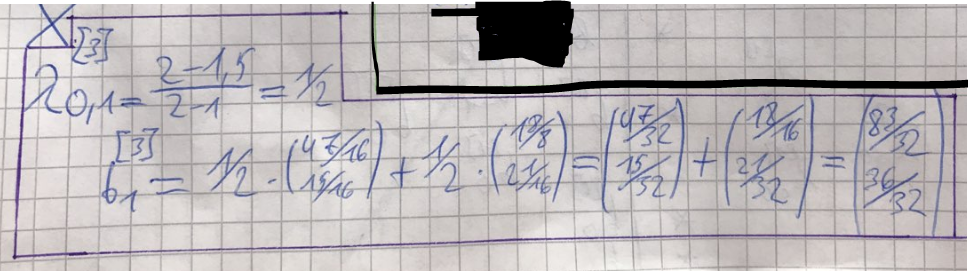
\includegraphics[scale=0.5]{1b)4.PNG}
\\
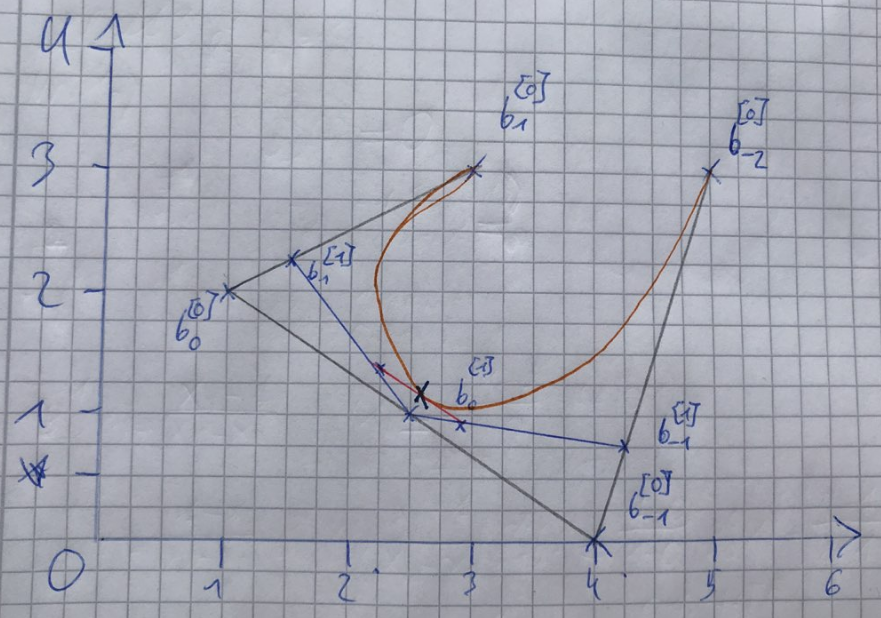
\includegraphics[scale=0.5]{1b)5.PNG}